%!TEX root = ../head.tex

\chapter{Übung}
\section{Einführung}
\subsection{}
\begin{enumerate}
	\item Datenformat inflexibel:
	\begin{enumerate}
		\item keine stand. Pfade
		\item viele Dateisys. erlauben keine Dateien über fixe Größe
		\item keine stand. Datentypen (.txt) und Schema der Datenspericherung leicht uneinheitl.
	\end{enumerate}
	\item mehrere Personen sollen/können darauf zugreifen
	\item Datenformat Abfragesprache/-tool auch neu "lernen" SQL einheitl.
	\item Redundanz sorgt für Anomalien (z.B. Aktualisierung d. Daten)
\end{enumerate}
\subsection{}
Rechteck: Entität, Raute: Bezeichner, Kreis: Attribute
\begin{enumerate}
	\item 3
	\item partielle Beziehungen
	\begin{itemize}
		\item SxT\(\to\)Ü
		\item ÜxT\(\to\)S
		\item SxÜ\(\to\)T
	\end{itemize}
	\item
	\begin{enumerate}
		\item Ein Tutor und ein Student nehmen an einer Übung teil
		\item An einer Übung mit einem Tutor nimmt ein Student teil
		\item Ein Student in einer Übung hat einen Tutor
	\end{enumerate}
	\item (1) und (3)
\end{enumerate}
\subsection{}
\begin{displaymath}
	A:N, C:M, B:1
\end{displaymath}
Faustregel: Auf der rechten Seite steht eine 1.
\subsection{}
ACHTUNG: Multiplizitäten genau andersrum wie bei 1.3
\begin{itemize}
	\item T:(1,*)
	\item Ü:(1,*)
	\item S:(0,1)
\end{itemize}
\subsection{}
\begin{itemize}
	\item Bahnhöfe M \(\leftrightarrow\) 1 Städte
	\item Bahnhöfe 1 \(\leftrightarrow\)verbindet\(\leftrightarrow\) 1 Bahnhöfe
	\item Bahnhöfe 1 \(\leftrightarrow\)verbindet\(\leftrightarrow\) N Züge
	\item Bahnhöfe 1 \(\leftrightarrow\)Start\(\leftrightarrow\) L Züge
	\item Bahnhöfe 1 \(\leftrightarrow\)Ziel\(\leftrightarrow\) K Züge
\end{itemize}

\section{ER-Modellierung}
\subsection{Prof-Stud}
\ref{img:Prof-Stud-ER}
\begin{figure}
	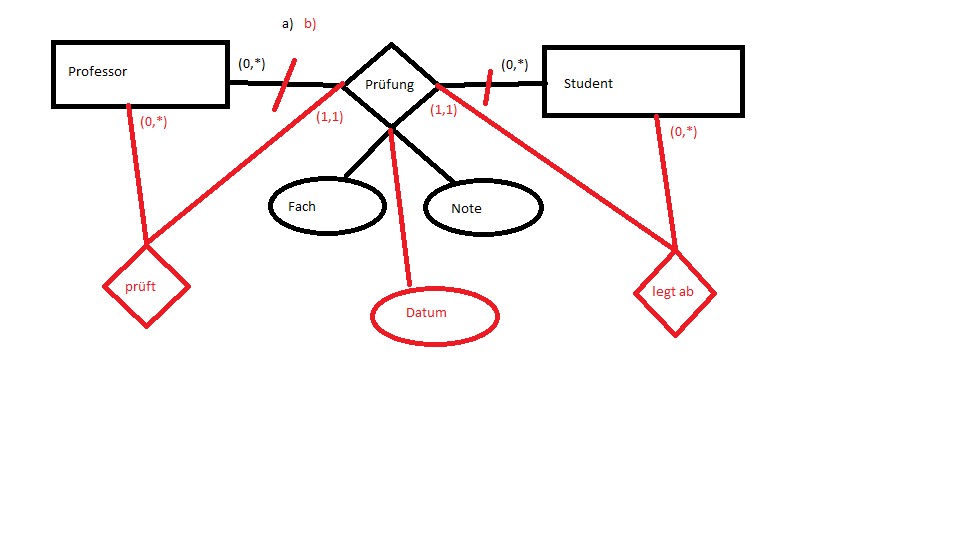
\includegraphics[width = 16cm]{./Database/Images/2_1.png}
	\caption{Professor-Student ER}
	\label{img:Prof-Stud-ER}
\end{figure}

\subsection{ER-Bahn}
\ref{img:Bahn-ER}
\begin{figure}
	\centering
	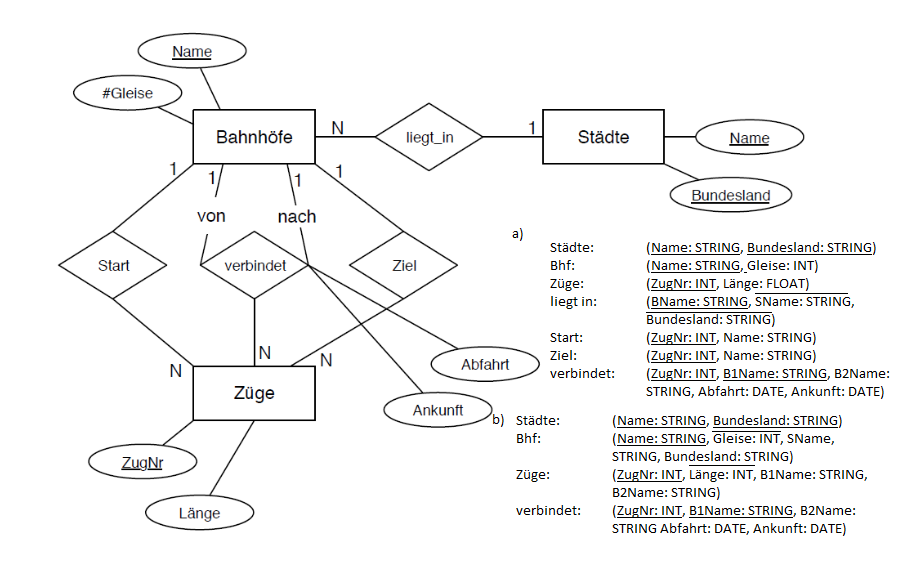
\includegraphics[width = 16cm]{./Database/Images/2_2.png}
	\caption{Bahnnetz ER}
	\label{img:Bahn-ER}
\end{figure}
\subsection{ER-Bsp}
\ref{img:Relations-ER}
\begin{figure}
	\centering
	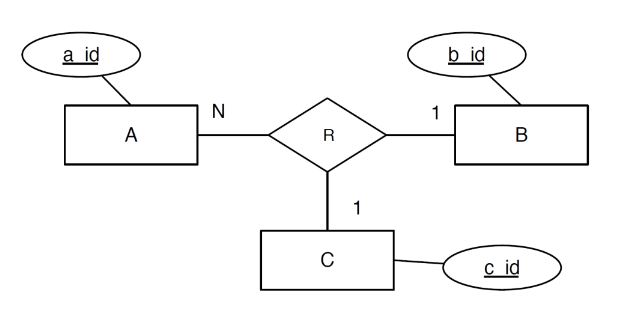
\includegraphics[width = 16cm]{./Database/Images/2_3a.png}
	\caption{Relations ER}
	\label{img:Relations-ER}
\end{figure}
\begin{enumerate}
	\item
	\begin{itemize}
		\item A x B \(\to\) C
		\item A x C \(\to\) B
	\end{itemize}
	\item
	\begin{itemize}
		\item A: (\underline{a id: INT})
		\item B: (\underline{b id: INT})
		\item C: (\underline{c id: INT})
	\end{itemize}
	\item
	\begin{itemize}
		\item \(R_1\): (\underline{a id}, \underline{b id}, c id)
		\item \(R_2\): (\underline{a id}, b id, \underline{c id})
	\end{itemize}
\end{enumerate}
\subsection{Vererbungshierarchie - Relationsschema }
\ref{img:Vererbungshierarchie}
\begin{figure}
	\centering
	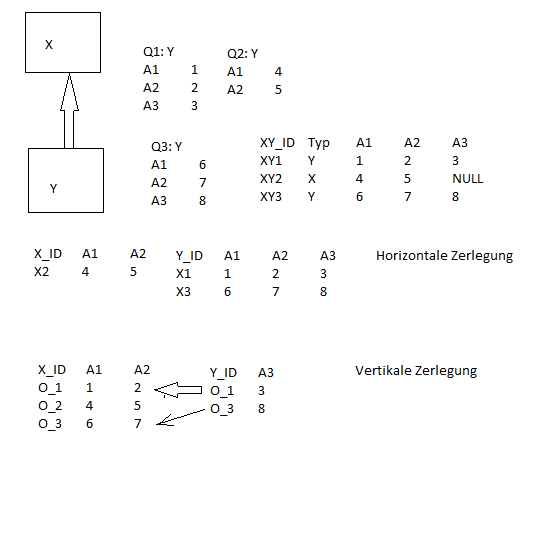
\includegraphics[width = 16cm]{./Database/Images/2_4.png}
	\caption{Relations ER}
	\label{img:Vererbungshierarchie}
\end{figure}

\section{Relationenalgebra}
dennis.koppenhagen@tu-dresden.de \\
\(\Pi\to\) Projektion, Spalte\\
\(\sigma\to\) Selektion, Zeile\\
\(\rho\to\) Umbenennung,\\
\subsection{}
\begin{enumerate}
	\item Geben Sie alle Vorlesungen an, die der Student X. gehört hat \\
	 \(R = \Pi_{\text{Titel, Vorl.Nr.}}\)(Vorlesung {\tiny \textifsym{|><|}} (hören {\tiny \textifsym{|><|}} \(\sigma_{\text{Name = X}}(\text{Studenten})\)))
	 \item Geben Sie die Titel der direkten Voraussetzungen für die Vorlesung Wissenschaftstheorie an:\\
	 \(R = \Pi_{\text{VVorg.Titel}}(\rho_{\text{VVrg}}(\text{Vorlesung })\){\tiny \textifsym{|><|}} \(_{\text{VVorg.VorlNr = Vorgänger}}\) \\ \((\)Voraussetzen {\tiny \textifsym{|><|}}  \(_{\text{VNach.Vorl.Nr = Nachf.}}(\sigma_{\text{VNach.Titel = 'Wiss.Theo'}}(\rho_{\text{VNach}}(\text{Vorlesungen})))))\)
	 \item 
	 \begin{align*}
	 		\Pi_{\text{S1.Name, S2.Name}}&\Biggl(\sigma_{\text{Titel = Grundzüge}}(\text{Vorlesung})\\
	 		&\text{ {\tiny \textifsym{|><|}} }_{\text{Vorl.Nr. = h1.Vorl.Nr}}\biggl((\rho_{\text{S1}}(\text{Studenten}))\\
	 		&\text{ {\tiny \textifsym{|><|}} }_{\text{S1.Matr.Nr = h1.Matr.Nr., S1.Matr.Nr != S2.Matr.Nr.}}\Big((\rho_{\text{h1}}(\text{hören}))\\
	 		&\text{ {\tiny \textifsym{|><|}} }_{\text{h1.Vorl = h2.VorlNr.}}(\rho_{h2}(\text{hören}))\Big)\\
	 		&\text{ {\tiny \textifsym{|><|}} }_{\text{S2.Matrikel = h2.Matrikel}} (\rho_{S2}(\text{Studenten}))\biggr)\Biggr)
	 \end{align*}
\end{enumerate}
\subsection{}
\begin{enumerate}
	\item Finden Sie die Assistenten von Professoren, die den Studenten Fichte unterrichtet haben, z.B. als potentielle Betreuer seiner Diplomarbeit
	\item Finden Sie die Studenten, die Vorlesungen hören (bzw. gehört haben), für die ihnen die direkten Voraussetzungen fehlen
\end{enumerate}
\subsection{}
\begin{enumerate}
	\item R {\tiny  \textifsym{|><|}} S
	\begin{tabularx}{\textwidth}{XXXXXX}	
	A	&B	&C	&D	&E	&G \\
	1	&1	&1	&1	&1	&3 \\
	2	&2	&3	&2	&3	&1 \\
	2	&3	&3	&2	&3	&1 \\
	\end{tabularx}
	\item R {\tiny  \textifsym{|><|d}} S
	\begin{tabularx}{\textwidth}{XXXXXX}	
	A	&B	&C	&D	&E	&G \\
	1	&1	&1	&1	&1	&3 \\
	2	&2	&3	&2	&3	&1 \\
	2	&3	&3	&2	&3	&1 \\
	NULL &NULL &1 &3 &2 &2 \\
	\end{tabularx}
	\item R {\tiny  \textifsym{d|><|d}} S
	\begin{tabularx}{\textwidth}{XXXXXX}	
	A	&B	&C	&D	&E	&G \\
	1	&1	&1	&1	&1	&3 \\
	2	&2	&3	&2	&3	&1 \\
	2	&3	&3	&2	&3	&1 \\
	NULL &NULL &1 &3 &2 &2 \\
	3	&2	&2	&3	&NULL &NULL \\
	\end{tabularx}
	\item R {\tiny  \textifsym{|><}} S
	\begin{tabularx}{\textwidth}{XXXX}	
	A	&B	&C	&D \\
	1	&1	&1	&1 \\
	2	&2	&3	&2 \\
	2	&3	&3	&2 \\
	\end{tabularx}
\end{enumerate}

\subsection{Kreuzprodukt und Divisionsoperator}
\begin{align*}
	&\Pi_A(R) &&= \{X,Y,Z\} \\
	&\Pi_A(R) \text{x} S &&= \{(X,2),(X,3),(Y,2),(y,3),(Z,2),(Z,3)\} \\
	&\Pi_A(R) x \S) - R &&= \{(X,3)\} \\
	&\Pi_A((\Pi_A (R)xS)-R) &&= \{X\} \\
	&\Pi_A(R) - \Pi_A (\ldots ) &&= \{Y,Z\}
\end{align*}

\section{SQL}
\subsection{Befehle in SQL}
\subsubsection{1}
\begin{lstlisting}
SELECT name,population
FROM city
ORDER BY population DESC
\end{lstlisting}
\subsubsection{2}
\begin{lstlisting}
SELECT city
FROM located
WHERE river IS NOT NULL
AND lake IS NOT NULL
\end{lstlisting}
\subsubsection{3}
\begin{lstlisting}
SELECT name,population
FROM city
WHERE country = 'D'
ORDER BY population DESC
\end{lstlisting}
\subsubsection{4}
\begin{lstlisting}
SELECT DISTINCT l.name 
FROM language l 
INNER JOIN encompasses e ON l.country = e.country
WHERE e.continent = 'Europe'
\end{lstlisting}
\subsubsection{5}
\begin{lstlisting}
fill
\end{lstlisting}
\subsubsection{8}
\begin{lstlisting}
SELECT DISTINCT c.name 
FROM country c
INNER JOIN city s ON s.country = c.code
INNER JOIN city hs ON c.capital = hs.name
WHERE s.population > hs.population
\end{lstlisting}
\subsubsection{9}
\begin{lstlisting}
SELECT c.name, SUM(s.population)
FROM city s
INNER JOIN country c ON s.country = c.code
WHERE s.population > 1000000
GROUP BY c.name
ORDER BY 2 DESC
\end{lstlisting}

\section{}
fill 16.05.
\subsection{Primzeugs}
\begin{enumerate}
\item Prim 1 \\
\begin{lstlisting}
SELECT p, p+2, p+4
FROM Prim
WHERE p + 2 in (SELECT p from PRIM)
	AND p + 4 in (SELECT p FROM PRIM)
\end{lstlisting}
\item Prim 2\\
\begin{lstlisting}
SELECT p
FROM Prim
WHERE ((p+1) mod 6 = 0 or (p-1) mod 6 = 0)
	AND p > 3
\end{lstlisting}
\end{enumerate}

\section{}
\subsection{ER-Modell}
MIN/MAX Angaben
\ref{img:MM}
\begin{figure}[h]
	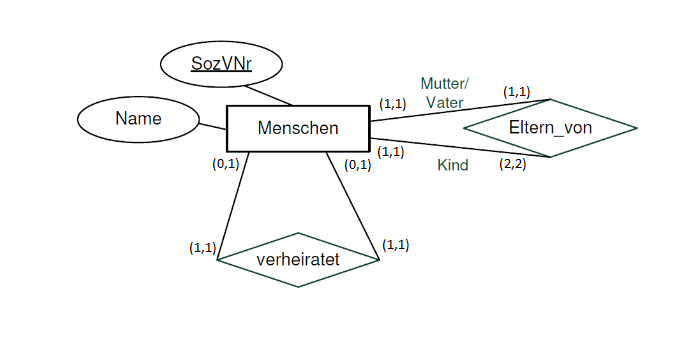
\includegraphics[width = 16cm]{./Database/Images/6_1.png}
	\caption{Min/Max}
	\label{img:MM}
\end{figure}
\begin{lstlisting}
CREATE TABLE Menschen (SozVNr varchar(30) primary key, 
	Name varchar(30));
\end{lstlisting}
verheiratet
\begin{lstlisting}
CREATE TABLE verheiratet(
	Ehepartner1 varchar(30) 
	REFERENCES Menschen ON DELETE CASCADE, 
	Eheparnter 2 varchar(30) NOT NULL UNIQUE
	REFERENCES Menschen ON DELETE CASCADE, PRIMARY KEY(Ehepartner1)
);
\end{lstlisting}
Eltern von
\begin{lstlisting}
CREATE TABLE Eltern_von (
	MutterVater varchar(30) NOT NULL REFERNECES Menschen, 
	Kind varchar(30) REFERNECES Menschen NOT NULL, 
	PRIMARY KEY(VaterMutter, Kind));
\end{lstlisting}
\subsection{SQL-Anfragen}
\begin{enumerate}
\item AB ist Schlüssel? Wenn ja dann darf folgendes keine Einträge haben.
\begin{lstlisting}
SELECT A,B FROM R GROUP BY A, B HAVING COUNT(*) > 1;
\end{lstlisting}
\item DE $\to$ B
\begin{lstlisting}
SELECT D, E FROM R GROPU BY D, E HAVING COUNT (DISTINCT B) > 1;
\end{lstlisting}
\end{enumerate}
\subsection{Relationsschema}
\begin{enumerate}
	\item
	\begin{itemize}
		\item \{Name, Aufbage\} $\to$ \{Erzielt\}
		\item \{Name \} $\to$ \{KlausurSumme, Bonus\}
		\item \{KNote, Bonus\} $\to$ \{Gnote\}
		\item \{KlausurSumme\} $\to$ \{KNote\}
		\item \{Aufgabe\} $\to$ \{Max\}
	\end{itemize}
\end{enumerate}
\section{06.06.2016}
\subsection{}
Attributhülle: $(F,A) = A^+$\\ Menge aller Attribute, die funktional von A bestimmt werden.
\subsubsection{Links-Reduktion}
$\forall \alpha \to \beta \in F: $ Wenn $\beta \subseteq $ Attributhülle $(F,(\alpha - A))$ dann entferne A auf linker Seite, $A \in \alpha$
\subsubsection{Rechts-Reduktion}
$\forall \alpha \to \beta \in F: $ Wenn B $ \in $ Attributhülle $(F\to(\alpha \to \beta) \cup (\alpha \to (\beta \to \text{ B}))\cup \alpha)$ dann entferne B auf rechter Seite, $B \in \beta$
\subsubsection{Aufgabe}
Beispiel Links- und Rechtsreduktion
\begin{align*}
F &= \{A \to B, B\to C, AB \to C\}\\
\text{nach Linksreduktion: }F &= \{A \to B, B\to C, A \to C\}\\
\text{nach Rechtsreduktion: }F &= \{A \to B, B \to C\, A \to \emptyset\}\\
&= \{A \to B, B \to C\} \text{ wird kanonische Überdeckung genannt}
\end{align*} 
\begin{enumerate}
	\item $\emptyset \to \{MaxSumme\}$
	\item FDS:
\begin{itemize}
	\item \{KNote, Bonus\} $\to$ \{GNote\}
	\item \{Aufgabe\} $\to$ \{Max\}
	\item \{ErzieltSumme\} $\to$ \{KNote\}
	\item \{Name, Aufgabe\} $\to$ \{Erzielt\}
	\item \{Name\} $\to$ \{ErzieltSumme, Bonus, GNote\} \\
		nach Rechtsreduktion: \{Name\} $\to$ \{ErzieltSumme, Bonus\}
	\item Formal funktioniert Reduktion so:\\
	\{Name\} $\to$ \{\underline{ErzieltSum}, Bonus, GNote\}\\
	\{ErzielstSum\} $\notin$ AttributHülle\{FD, F - \{Name\} $\to$ \{ErzieltSum, Bonus, GNote\} $\cup$ (\{Name\}$\to$\{Bonus,GNote\}),\{Name\}),
	\end{itemize}
	\item
	\begin{itemize}
		\item Noten: \{[\underline{KNote},\underline{Bonus}, GNote]\}
		\item Aufgaben: \{[\underline{Aufgabe}, Max]\}
		\item PunkteNote: \{[ES, KNote]\}
		\item MaxSumme: \{[MaxSumme]\}
	\end{itemize}
\end{enumerate}
\subsection{}
\begin{itemize}
	\item \{Signatur\} $\to$ \{Titel\}
	\item \{Vorgang\} $\to$ \{Datum\}
	\item \{Datum,Vorgang\} $\to$\{Benutzer\}
	\item \{Benutzer\} $\to$ \{Straße, PLZ, Ort\}
	\item \{PLZ\} $\to$ \{Ort\}
\end{itemize}
PK: \{Vorgang, Signatur\}
\begin{itemize}
	\item R1: \{\underline{Vorgang}, Datum, Benutzer, Straße, PLZ, Ort\}
	\item R2: \{\underline{Signatur}, Titel\}
	\item R3: \{\underline{Vorgang}, \underline{Signatur}\}
\end{itemize}
ist in 2. NF
\subsection{FLüge}
\begin{itemize}
	\item[] FLÜGE(E,G,A0,Z0,AZ,D)
	\item[] ReiseBüros(\underline{K},N,O,A)
	\item[] Passagiere(\underline{V},\underline{N},W)
	\item[] Reserviert(\underline{K}, \underline{F})
	\item[] BuchtBei(\underline{V},\underline{N}, \underline{K})
	\item[] FliegtMit(\underline{V}, \underline{N}, \underline{F})
	\item[] $ F^+ = F \cup G \cup A0 \cup Z0 \cup AZ \cup D$
	\item[] $ G\cup A0 \cup Z0)^+ = G \cup A0 \cup Z0\cup F \cup AZ \cup D $
	\item[] $ G\cup A0 \cup Z0 \to F$
\end{itemize}
\section{}
\subsection{}
\begin{itemize}
	\item[A]tomicity
	\item[C]onsistency
	\item[I]solation
	\item[D]urability
\end{itemize}
\subsection{}
\subsubsection{DIRTY READ}
\begin{tabularx}{\textwidth}{|X|X|}
\hline
	T2 & T3\\
\hline
 & B0T3\\
\hline
& r2(B)\\
\hline
& w3(B)\\
\hline
B0T2&\\
\hline
r2(B)&\\
\hline
r2(A)&\\
\hline
w2(B)&\\
\hline
C2&\\
\hline
&a3\\
\hline
\end{tabularx}
\subsubsection{NON REPEATABLE READ}
\begin{tabularx}{\textwidth}{|X|X|}
\hline
	T1 & T2\\
\hline
 B0T1&\\
\hline
 r1(B)&\\
\hline
& B0T2\\
\hline
&r2(B)\\
\hline
&r2(A)\\
\hline
&w2(B)\\
\hline
&C2\\
\hline
w1(A)&\\
\hline
r1(B)&\\
\hline
w1(B) & \\
\hline
C1&\\
\hline
\end{tabularx}

\subsection{}
\begin{enumerate}
	\item \ldots
	\item Serialisierbarkeitsgraph
	\begin{itemize}
		\item T1
		\begin{itemize}
			\item T1 $\to$ T2
			\item T1 $\to$ T3	
		\end{itemize}
		\item T2
		\begin{itemize}
			\item T2 $\to$ T1
			\item T2 $\to$ T3
		\end{itemize}
		\item T3
	\end{itemize}
	\item ist nicht serialisierbar ($\exists$ Zyklen)
\end{enumerate}

\subsection{}
\begin{enumerate}
	\item w1[x]w1[y]c1r2[x]w2[z]c2r3[y]a3
	\begin{enumerate}
		\item SR (keine Zyklen)?
		\begin{itemize}
			\item T1
			\begin{itemize}
				\item T1 $\to$ T2
				\item T1 $\to$ T3
			\end{itemize}
			\item T2
			\item T3
		\end{itemize}
		$\Rightarrow$ der Graph hat keine Zyklen
	\item RC: schreib-lese Reihenfolge = schließ Reihenfolge
	\begin{itemize}
		\item[ja] $\to$ ACA: Lesen nur von abgeschlossenen Transaktionen
		\begin{itemize}
			\item[ja] $\to$ ST: Schreiben nur auf abgeschlossenen Transaktionen
		\end{itemize}
	\end{itemize}
	\end{enumerate}
	\item
	\item 
	\begin{itemize}
			\item T1
			\begin{itemize}
				\item T1 $\to$ T2
				\item T1 $\to$ T3
			\end{itemize}
			\item T2
			\begin{itemize}
				\item T2 $\to$ T1 $\Rightarrow$ ZYKLUS!!! Schreib-Lese-Reihenfolge?
				\begin{itemize}
					\item nicht RC $\to$ nicht ACA und nicht ST
				\end{itemize}
			\end{itemize}
			\item T3
	\end{itemize}
\end{enumerate}

\subsection{}
\begin{enumerate}
	\item $w_1(x)r_2(x)w_2(y)c_2c_1$ Historie nicht rücksetzbar aber korrekt bei 2PL $\to$ deshalb S2PL, damit wird der Term serialisierbar
	\item S2PL erzeugt serielle Abläufe, dagegen 2PL serialisierbar aber \textbf{ohne} serielle Abläufe zu garantieren!!
\end{enumerate}
\begin{tabularx}{\textwidth}{X|X}
T1 &T2\\
\hline
B0T1&- \\
Lock X(A) &- \\
w1&-\\
\hline
-&B0T2\\
-&Lock X(B)\\
-&W2(B)\\
\hline
Lock S(B) &-\\
-&Lock S(A)
\end{tabularx}

\subsection{}
\begin{tabularx}{\textwidth}{|X|X|X|X|X|X|X|}
\hline
&a &b &c &d &e &f\\
\hline
T1 &x &s &\textbf{X} &- &s &-\\
\hline
T2 &- &s &- &- &- &\textbf{S}\\
\hline
T3 &- &\textbf{X} &s &- &s &-\\
\hline
T4 &\textbf{S} &- &s &x &s &-\\
\hline
T5 &- &- &- &\textbf{X} &- &x\\
\hline
\end{tabularx}
\begin{itemize}
	\item T1
	\begin{itemize}
		\item T1 $\to$ T3
		\item T1 $\to$ T4
	\end{itemize}
	\item T2
	\begin{itemize}
		\item T2 $\to$ T5
	\end{itemize}
	\item T3
	\begin{itemize}
		\item T3 $\to$ T1
		\item T3 $\to$ T2
	\end{itemize}
	\item T4
	\begin{itemize}
		\item T4 $\to$ T1
	\end{itemize}
	\item T5
	\begin{itemize}
		\item T5 $\to$ T4
	\end{itemize}
\end{itemize}